\chapter{Souřadné systémy}

V~této příloze jsou vyjádřeny operace v~bežně používaných souřadných systémech.

\section{Kartézský souřadný systém}

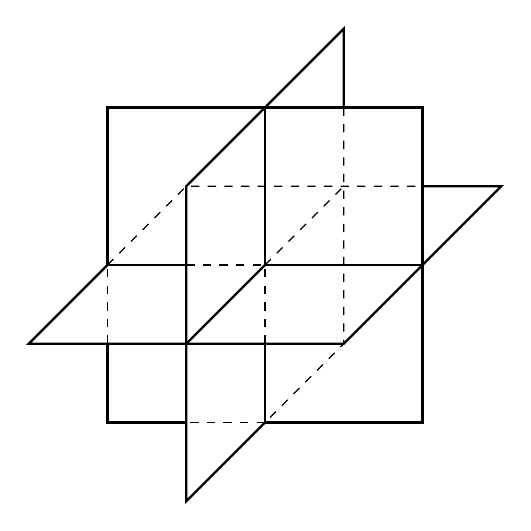
\begin{tikzpicture}

\drawaxes{0}{0}{6}{4}{2}

% Rovina XY
\draw[thick] (0, -1) -- (-1, -1) -- (-1, 0);
\draw[dashed] (-1, 0) -- (-1, 1);
\draw[thick] (-1, 1) -- (-1, 3) -- (3, 3) -- (3, -1) -- (1, -1);
\draw[dashed] (1, -1) -- (0, -1);

% Rovina YZ
\draw[thick] (3, 2) -- (4, 2) -- (2, 0) -- (-2, 0) -- (-1, 1);
\draw[dashed] (-1, 1) -- (0, 2) -- (3, 2);

% Rovina XZ
\draw[thick] (1, -1) -- (0, -2) -- (0, 2) -- (2, 4) -- (2, 3);
\draw[dashed] (2, 3) -- (2, 0) -- (1, -1);

% X
\draw[thick] (-1, 1) -- (0, 1);
\draw[dashed] (0, 1) -- (1, 1);
\draw[thick] (1, 1) -- (3, 1);

% Y
\draw[thick] (0, 0) -- (1, 1);
\draw[dashed] (1, 1) -- (2, 2);

% Z
\draw[thick] (1, -1) -- (1, 0);
\draw[dashed] (1, 0) -- (1, 1);
\draw[thick] (1, 1) -- (1, 3);

\end{tikzpicture}


\begin{equation}
\begin{split}
P = P' = (x, y, z)
\end{split}
\end{equation}

\begin{equation}
\begin{split}
\frac{\partial p'_j}{\partial P_i} = \frac{\partial p_j}{\partial P'_i} = \delta_{ij}
\end{split}
\end{equation}

\begin{equation}
\begin{split}
g_{jk} = g^{jk} = \delta_{ij}
\end{split}
\end{equation}

\begin{equation}
\begin{split}
\frac{\partial^2 p_j}{\partial P'^2_i} = 0
\end{split}
\end{equation}

\begin{equation}
\begin{split}
\sum_{i=1}^3 \frac{\partial^2 p_j}{\partial P'^2_i} = 0
\end{split}
\end{equation}

\begin{equation}
\label{eq:kartezsky_ss_div}
\diverg{\kovarvect{v}} = \frac{\partial v_x}{\partial x} + \frac{\partial v_y}{\partial y} + \frac{\partial v_z}{\partial z}\end{equation}

\begin{equation}
\label{eq:kartezsky_ss_laplace}
\Delta \varphi = \frac{\partial^2 \varphi}{\partial x^2} + \frac{\partial^2 \varphi}{\partial y^2} + \frac{\partial^2 \varphi}{\partial x^2}\end{equation}

\begin{equation}
\label{eq:kartezsky_ss_j}
J = J' = 1
\end{equation}

\begin{equation}
\label{eq:kartezsky_ss_rotace}
\rot \kovarvect{v} = \left(\frac{\partial v_z}{\partial y} - \frac{\partial v_y}{\partial z}, \frac{\partial v_x}{\partial z} - \frac{\partial v_z}{\partial x}, \frac{\partial v_y}{\partial x} - \frac{\partial v_x}{\partial y} \right)
\end{equation}

\section{Polární souřadný systém}

\begin{equation}
\begin{split}
P' = (x, y) \\
P = (r, \alpha)
\end{split}
\end{equation}

\begin{equation}
\begin{split}
x = p'_1(r, \alpha) = r \cdot \cos \alpha \\
y = p'_2(r, \alpha) = r \cdot \sin \alpha
\end{split}
\end{equation}

\begin{equation}
\begin{split}
r = p_1(x, y) = \sqrt{x^2 + y^2} \\
\alpha = p_2(x, y) = \arctg \frac{y}{x}
\end{split}
\end{equation}

\begin{tabular}{| c || c | c |}
\hline
\(\frac{\partial p'_j}{\partial P_i}\) & \(i=1\) & \(i=2\) \\
\hline
\hline
\(j=1\) & \(\frac{\partial x}{\partial r} = \cos \alpha\) & \(\frac{\partial x}{\partial \alpha} = -r \cdot \sin \alpha\) \\
\hline
\(j=2\) & \(\frac{\partial y}{\partial r} = \sin \alpha\) & \(\frac{\partial y}{\partial \alpha} = r \cdot \cos \alpha\) \\
\hline
\end{tabular}

\begin{tabular}{| c || c | c |}
\hline
\(\frac{\partial p_j}{\partial P'_i}\) & \(i=1\) & \(i=2\) \\
\hline
\hline
\(j=1\) & \(\frac{\partial r}{\partial x} = \cos \alpha\) & \(\frac{\partial r}{\partial y} = \sin \alpha\) \\
\hline
\(j=2\) & \(\frac{\partial \alpha}{\partial x} = -\frac{\sin \alpha}{r}\) & \(\frac{\partial \alpha}{\partial y} = \frac{\cos \alpha}{r}\) \\
\hline
\end{tabular}

\begin{tabular}{| c || c | c |}
\hline
\(g_{jk}\) & \(j=1\) & \(j=2\) \\
\hline
\hline
\(k=1\) & \(1\) & \(0\) \\
\hline
\(k=2\) & \(0\) & \(r^2\) \\
\hline
\end{tabular}

\begin{tabular}{| c || c | c |}
\hline
\(g^{jk}\) & \(j=1\) & \(j=2\) \\
\hline
\hline
\(k=1\) & \(1\) & \(0\) \\
\hline
\(k=2\) & \(0\) & \(\frac{1}{r^2}\) \\
\hline
\end{tabular}

\begin{tabular}{| c || c | c |}
\hline
\(\frac{\partial^2 p_j}{\partial P'^2_i}\) & \(i=1\) & \(i=2\) \\
\hline
\hline
\(j=1\) & \(\frac{\partial^2 r}{\partial x^2} = \frac{\sin^2 \alpha}{r}\) & \(\frac{\partial^2 r}{\partial y^2} = \frac{\cos^2 \alpha}{r}\) \\
\hline
\(j=2\) & \(\frac{\partial^2 \alpha}{\partial x^2} = \frac{\sin 2\alpha}{r^2}\) & \(\frac{\partial^2 \alpha}{\partial y^2} = -\frac{\sin 2\alpha}{r^2}\) \\
\hline
\end{tabular}

\begin{tabular}{| c || c | c |}
\hline
\(j\) & \(1\) & \(2\) \\
\hline
\hline
\(\sum_{i=1}^2 \frac{\partial^2 p_j}{\partial P'^2_i}\) & \(\frac{1}{r}\) & 0 \\
\hline
\end{tabular}

\begin{equation}
\label{eq:polarni_ss_div}
\diverg{\kovarvect{v}} = \frac{\partial v_r}{\partial r} + \frac{1}{r^2} \frac{\partial v_{\alpha}}{\partial \alpha} + \frac{v_r}{r}
\end{equation}

\begin{equation}
\label{eq:polarni_ss_laplace}
\Delta \varphi = \frac{\partial^2 \varphi}{\partial r^2} + \frac{1}{r^2} \frac{\partial^2 \varphi}{\partial \alpha^2} + \frac{\partial \varphi}{\partial r}
\end{equation}

\begin{equation}
\label{eq:polarni_ss_j}
J = r
\end{equation}

\begin{equation}
\label{eq:polarni_ss_j_inv}
J' = \frac{1}{r}
\end{equation}


\section{Cylindrický souřadný systém}

\begin{equation}
\begin{split}
P' = (x, y, z) \\
P = (r, \alpha, z)
\end{split}
\end{equation}

\begin{equation}
\begin{split}
x = p'_1(r, \alpha, z) = r \cdot \cos \alpha \\
y = p'_2(r, \alpha, z) = r \cdot \sin \alpha \\
z = p'_3(r, \alpha, z) = z
\end{split}
\end{equation}

\begin{equation}
\begin{split}
r = p_1(x, y, z) = \sqrt{x^2 + y^2} \\
\alpha = p_2(x, y, z) = \arctg \frac{y}{x} \\
z = p_3(x, y, z) = z
\end{split}
\end{equation}

\begin{tabular}{| c || c | c | c |}
\hline
\(\frac{\partial p'_j}{\partial P_i}\) & \(i=1\) & \(i=2\) & \(i=3\) \\
\hline
\hline
\(j=1\) & \(\frac{\partial x}{\partial r} = \cos \alpha\) & \(\frac{\partial x}{\partial \alpha} = -r \cdot \sin \alpha\) & \(\frac{\partial x}{\partial z} = 0\) \\
\hline
\(j=2\) & \(\frac{\partial y}{\partial r} = \sin \alpha\) & \(\frac{\partial y}{\partial \alpha} = r \cdot \cos \alpha\) & \(\frac{\partial y}{\partial z} = 0\) \\
\hline
\(j=3\) & \(\frac{\partial y}{\partial r} = 0\) & \(\frac{\partial y}{\partial \alpha} = 0\) & \(\frac{\partial z}{\partial z} = 1\) \\
\hline
\end{tabular}

\begin{tabular}{| c || c | c | c |}
\hline
\(\frac{\partial p_j}{\partial P'_i}\) & \(i=1\) & \(i=2\) & \(i=3\)\\
\hline
\hline
\(j=1\) & \(\frac{\partial r}{\partial x} = \cos \alpha\) & \(\frac{\partial r}{\partial y} = \sin \alpha\) & \(\frac{\partial r}{\partial z} = 0\)\\
\hline
\(j=2\) & \(\frac{\partial \alpha}{\partial x} = -\frac{\sin \alpha}{r}\) & \(\frac{\partial \alpha}{\partial y} = \frac{\cos \alpha}{r}\) & \(\frac{\partial \alpha}{\partial z} = 0\)\\
\hline
\(j=3\) & \(\frac{\partial \alpha}{\partial x} = 0\) & \(\frac{\partial \alpha}{\partial y} = 0\) & \(\frac{\partial z}{\partial z} = 1\)\\
\hline
\end{tabular}

\begin{tabular}{| c || c | c | c |}
\hline
\(g_{jk}\) & \(j=1\) & \(j=2\) & \(j=3\) \\
\hline
\hline
\(k=1\) & \(1\) & \(0\) & \(0\) \\
\hline
\(k=2\) & \(0\) & \(r^2\) & \(0\) \\
\hline
\(k=3\) & \(0\) & \(0\) & \(1\) \\
\hline
\end{tabular}

\begin{tabular}{| c || c | c | c |}
\hline
\(g^{jk}\) & \(j=1\) & \(j=2\) & \(j=3\) \\
\hline
\hline
\(k=1\) & \(1\) & \(0\) & \(0\) \\
\hline
\(k=2\) & \(0\) & \(\frac{1}{r^2}\) & \(0\) \\
\hline
\(k=3\) & \(0\) & \(0\) & \(1\) \\
\hline
\end{tabular}

\begin{tabular}{| c || c | c | c |}
\hline
\(\frac{\partial^2 p_j}{\partial P'^2_i}\) & \(i=1\) & \(i=2\) & \(i=3\) \\
\hline
\hline
\(j=1\) & \(\frac{\partial^2 r}{\partial x^2} = \frac{\sin^2 \alpha}{r}\) & \(\frac{\partial^2 r}{\partial y^2} = \frac{\cos^2 \alpha}{r}\) & \(\frac{\partial^2 r}{\partial z^2} = 0\) \\
\hline
\(j=2\) & \(\frac{\partial^2 \alpha}{\partial x^2} = \frac{\sin 2 \alpha}{r^2}\) & \(\frac{\partial^2 \alpha}{\partial y^2} = -\frac{\sin 2\alpha}{r^2}\) & \(\frac{\partial^2 \alpha}{\partial z^2} = 0\) \\
\hline
\(j=3\) & \(\frac{\partial^2 z}{\partial x^2} = 0\) & \(\frac{\partial^2 z}{\partial y^2} = 0\) & \(\frac{\partial^2 z}{\partial z^2} = 0\) \\
\hline
\end{tabular}


\begin{tabular}{| c || c | c | c |}
\hline
\(j\) & \(1\) & \(2\) & \(3\) \\
\hline
\hline
\(\sum_{i=1}^3 \frac{\partial^2 p_j}{\partial P'^2_i}\) & \(\frac{1}{r}\) & 0 & 0 \\
\hline
\end{tabular}

\begin{equation}
\label{eq:cylindricky_ss_div}
\diverg{\kovarvect{v}} = \frac{\partial v_r}{\partial r} + \frac{1}{r^2} \frac{\partial v_{\alpha}}{\partial \alpha} + \frac{\partial v_z}{\partial z} + \frac{v_r}{r}
\end{equation}

\begin{equation}
\label{eq:cylindricky_ss_laplace}
\Delta \varphi = \frac{\partial^2 \varphi}{\partial r^2} + \frac{1}{r^2} \frac{\partial^2 \varphi}{\partial \alpha^2} + \frac{\partial^2 \varphi}{\partial z^2} + \frac{\partial \varphi}{\partial r}
\end{equation}

\begin{equation}
\label{eq:cylindricky_ss_j}
J = r
\end{equation}

\begin{equation}
\label{eq:cylindricky_ss_j_inv}
J' = \frac{1}{r}
\end{equation}

\begin{equation}
\label{eq:cylindricky_ss_rotace}
\kontravect{u} = \rot \kovarvect{v} = \frac{1}{r} \cdot \left( \frac{\partial v_{z}}{\partial \alpha} - \frac{\partial v_{\alpha}}{\partial z}, \frac{\partial v_{r}}{\partial z} - \frac{\partial v_{z}}{\partial r}, \frac{\partial v_{\alpha}}{\partial r} - \frac{\partial v_{r}}{\partial \alpha} \right)
\end{equation}


\section{Sférický souřadný systém}

\begin{equation}
\begin{split}
P' = (x, y, z) \\
P = (r, \alpha, \beta)
\end{split}
\end{equation}

\begin{equation}
\begin{split}
x = p'_1(r, \alpha, \beta) = r \cdot \cos \alpha \cdot \cos \beta \\
y = p'_2(r, \alpha, \beta) = r \cdot \sin \alpha \cdot \cos \beta \\
z = p'_3(r, \alpha, \beta) = r \cdot \sin \beta
\end{split}
\end{equation}

\begin{equation}
\begin{split}
r = p_1(x, y, z) = \sqrt{x^2 + y^2 + z^2} \\
\alpha = p_2(x, y, z) = \arctg \frac{y}{x} \\
\beta = p_3(x, y, z) = \arctg \frac{z}{\sqrt{x^2 + y^2}}
\end{split}
\end{equation}

\begin{tabular}{| c || c | c | c |}
\hline
\(\frac{\partial p'_j}{\partial P_i}\) & \(i=1\) & \(i=2\) & \(i=3\) \\
\hline
\hline
\(j=1\) & \(\frac{\partial x}{\partial r} = \cos \alpha \cdot \cos \beta\) & \(\frac{\partial x}{\partial \alpha} = -r \cdot \sin \alpha \cdot \cos \beta\) & \(\frac{\partial x}{\partial \beta} = -r \cdot \cos \alpha \cdot \sin \beta\) \\
\hline
\(j=2\) & \(\frac{\partial y}{\partial r} = \sin \alpha \cdot \cos \beta\) & \(\frac{\partial y}{\partial \alpha} = r \cdot \cos \alpha \cdot \cos \beta\) & \(\frac{\partial y}{\partial \beta} = -r \cdot \sin \alpha \cdot \sin \beta\) \\
\hline
\(j=3\) & \(\frac{\partial z}{\partial r} = \sin \beta\) & \(\frac{\partial z}{\partial \alpha} = 0\) & \(\frac{\partial z}{\partial \beta} = r \cdot \cos \beta\) \\
\hline
\end{tabular}

\begin{tabular}{| c || c | c | c |}
\hline
\(\frac{\partial p_j}{\partial P'_i}\) & \(i=1\) & \(i=2\) & \(i=3\)\\
\hline
\hline
\(j=1\) & \(\frac{\partial r}{\partial x} = \cos \alpha \cdot \cos \beta\) & \(\frac{\partial r}{\partial y} = \sin \alpha \cdot \cos \beta\) & \(\frac{\partial r}{\partial z} = \sin \beta\)\\
\hline
\(j=2\) & \(\frac{\partial \alpha}{\partial x} = -\frac{\sin \alpha}{r \cdot \cos \beta}\) & \(\frac{\partial \alpha}{\partial y} = \frac{\cos \alpha}{r \cdot \cos \beta}\) & \(\frac{\partial \alpha}{\partial z} = 0\)\\
\hline
\(j=3\) & \(\frac{\partial \beta}{\partial x} = \frac{-\cos \alpha \cdot \sin \beta}{r}\) & \(\frac{\partial \beta}{\partial y} = \frac{-\sin \alpha \cdot  \sin \beta}{r}\) & \(\frac{\partial \beta}{\partial z} = \frac{\cos \beta}{r}\)\\
\hline
\end{tabular}


\begin{tabular}{| c || c | c | c |}
\hline
\(g_{jk}\) & \(j=1\) & \(j=2\) & \(j=3\) \\
\hline
\hline
\(k=1\) & \(1\) & \(0\) & \(0\) \\
\hline
\(k=2\) & \(0\) & \(r^2 \cdot \cos^2 \beta\) & \(0\) \\
\hline
\(k=3\) & \(0\) & \(0\) & \(r^2\) \\
\hline
\end{tabular}

\begin{tabular}{| c || c | c | c |}
\hline
\(g^{jk}\) & \(j=1\) & \(j=2\) & \(j=3\) \\
\hline
\hline
\(k=1\) & \(1\) & \(0\) & \(0\) \\
\hline
\(k=2\) & \(0\) & \(\frac{1}{r^2 \cdot \cos^2 \beta}\) & \(0\) \\
\hline
\(k=3\) & \(0\) & \(0\) & \(\frac{1}{r^2}\) \\
\hline
\end{tabular}

\begin{tabular}{| c || c | c | c |}
\hline
\(\frac{\partial^2 p_j}{\partial P'^2_i}\) & \(i=1\) & \(i=2\) & \(i=3\) \\
\hline
\hline
\(j=1\) & \(\frac{\partial^2 r}{\partial x^2} = \frac{\sin^2 \alpha + \cos^2 \alpha \cdot \sin^2 \beta}{r}\) & \(\frac{\partial^2 r}{\partial y^2} = \frac{\cos^2 \alpha + \sin^2 \alpha \cdot \sin^2 \beta}{r}\) & \(\frac{\partial^2 r}{\partial z^2} = \frac{\cos^2 \beta}{r}\) \\
\hline
\(j=2\) & \(\frac{\partial^2 \alpha}{\partial x^2} = \frac{\sin 2\alpha}{r^2 \cdot \cos^2 \beta}\) & \(\frac{\partial^2 \alpha}{\partial y^2} = -\frac{\sin 2\alpha}{r^2 \cdot \cos^2 \beta}\) & \(\frac{\partial^2 \alpha}{\partial z^2} = 0\) \\
\hline
\(j=3\) & \(\frac{\partial^2 \beta}{\partial x^2} = \frac{\cos^2 \alpha \cdot \sin 2 \beta - \sin^2 \alpha \cdot \tg \beta}{r^2}\) & \(\frac{\partial^2 \beta}{\partial y^2} = \frac{\sin^2 \alpha \cdot \sin 2 \beta - \cos^2 \alpha \cdot \tg \beta}{r^2}\) & \(\frac{\partial^2 \beta}{\partial z^2} = -\frac{\sin 2 \beta}{r^2}\) \\
\hline
\end{tabular}

\begin{tabular}{| c || c | c | c |}
\hline
\(j\) & \(1\) & \(2\) & \(3\) \\
\hline
\hline
\(\sum_{i=1}^3 \frac{\partial^2 p_j}{\partial P'^2_i}\) & \(\frac{2}{r}\) & 0 & \(-\frac{\tg \beta}{r^2}\) \\
\hline
\end{tabular}

\begin{equation}
\label{eq:sfericky_ss_div}
\diverg{\kovarvect{v}} = \frac{\partial v_r}{\partial r} + \frac{1}{r^2 \cdot \cos^2 \beta} \frac{\partial v_{\alpha}}{\partial \alpha} + \frac{1}{r^2} \frac{\partial v_{\beta}}{\partial \beta} + \frac{2 \cdot v_r}{r} - \frac{\tg \beta \cdot v_{\beta}}{r^2}
\end{equation}

\begin{equation}
\label{eq:sfericky_ss_div}
\Delta \varphi = \frac{\partial^2 \varphi}{\partial r^2} + \frac{1}{r^2 \cdot \cos^2 \beta} \frac{\partial^2 \varphi}{\partial \alpha^2} + \frac{1}{r^2} \frac{\partial^2 \varphi}{\partial \beta^2} + \frac{2}{r} \cdot \frac{\partial \varphi}{\partial r} - \frac{\tg \beta}{r^2} \cdot \frac{\partial \varphi}{\partial \beta}
\end{equation}

\begin{equation}
\label{eq:sfericky_ss_j}
J = r^2 \cdot \cos \beta
\end{equation}

\begin{equation}
\label{eq:sfericky_ss_j_inv}
J' = \frac{1}{r^2 \cdot \cos \beta}
\end{equation}

\begin{equation}
\label{eq:sfericky_ss_rotace}
\kontravect{u} = \rot \kovarvect{v} = \frac{1}{r^2 \cdot \cos \beta} \cdot \left( \frac{\partial v_{\beta}}{\partial \alpha} - \frac{\partial v_{\alpha}}{\partial \beta}, \frac{\partial v_{r}}{\partial \beta} - \frac{\partial v_{\beta}}{\partial r}, \frac{\partial v_{\alpha}}{\partial r} - \frac{\partial v_{r}}{\partial \alpha} \right)
\end{equation}
